\documentclass{hipatia}
\usepackage{tkz-euclide}
\tkzSetUpLine[line width=1.25pt]
\tkzSetUpPoint[size=3pt]

%Use \DeclareMathOperator para definir novos
% operadores para o modo matemático
\DeclareMathOperator{\sen}{sen}

%Evite numerar teoremas
%Prefira nomeá-los
%Use os ambientes abaixo
\newtheorem*{theorem*}{Teorema}
\newtheorem*{lemma*}{Lema}

% Evite títulos muito longos
\title{O Farol de Euclides}
% Se for necessário diminuir a fonte do título 
% para caber no quadro, use
% \title{ \fontsize{28}{28}\selectfont Uma Nova Demonstração do\\  \fontsize{28}{28}\selectfont Teorema de Pitágoras}

% O Subtítulo é o nome da seção da revista
% Deve ser uma palavra de origem grega
\subtitle{História}
\author{Vinícius Mello}
% A data não é necessária
%\date{October 2023}
% Não se preocupe com a numeração
% das páginas ou com o número da edição

\begin{document}
\setcounter{page}{\historiapage}
\maketitle

\section{Introdução}

No início do ano de 2024, fui convidado a proferir
a primeira palestra do ano do Seminário Café
Cultural, evento tradicional do Departamento de
Matemática da UFBA. Como estava, naquele momento,
revisando material para a disciplina ``Geometria
Euclidiana Plana'' que lecionaria no primeiro
semestre (creio que pela décima vez, mas sem nunca
ter ficado plenamente satisfeito, devo confessar),
pensei inicialmente em discorrer sobre um tópico
qualquer de Geometria Euclidiana.

Mas a pesquisa que estava fazendo para atualizar
meu material de ensino me fez descobrir tantos
artigos recentes que ou versavam especificamente
sobre \emph{Os Elementos},  obra máxima de Euclides
de Alexandria, ou que ao menos se referiam a ela
sempre  nos termos mais elevados, ainda que
tratassem de temas atualíssimos, como Inteligência
Artificial ou Demonstração Automática de Teoremas,
que tive um lampejo: embora o Farol de Alexandria,
maravilha da antiguidade construída na mesma época
em que \emph{Os Elementos} foi escrito, tenha já se
apagado há muito tempo, o ``Farol de Euclides'',
ou seja, \emph{Os Elementos}, nunca deixou de nos
iluminar nesses mais de dois mil e trezentos anos! 

Foi esse o mote usado para organizar minha
palestra. Na oportunidade, posso dizer que obtive
sucesso no Seminário, embora tenha sido
superficial em alguns momentos, devido ao tempo
curto. Aproveito esta oportunidade, aqui na
\textsc{Revista de Matemática Hipátia}, para
transformar aquela palestra em um artigo de
divulgação, mantendo a mesma estrutura, mas me
aprofundando um pouco mais em alguns pontos. Após
uma breve exposição do contexto histórico no qual
Euclides viveu e do conteúdo dos \emph{Elementos},
discutiremos o que realmente Euclides estava
tentando fazer, sempre atentos ao perigo do
anacronismo, e depois passearemos por vários
momentos nos quais a luz do Farol de Euclides se
projetou na história da Matemática.  


\section{O Nome}

O título ``Elementos'' (\emph{Stoicheía}, em grego)
 carrega uma profundidade
conceitual que transcende sua aparente
simplicidade, evocando uma reflexão sobre os
fundamentos do conhecimento geométrico. A
etimologia da palavra grega \emph{stoicheion}
(elemento) revela uma multiplicidade de
significados que enriquecem a interpretação do
tema. Segundo De Simone \cite{deSimone2020},
 \emph{stoicheion} pode se referir a uma
letra do alfabeto, representando os componentes
básicos da escrita, a uma forma geométrica
simples ou, ainda, aos elementos físicos
clássicos --- terra, ar, fogo e água --- conforme
a tradição filosófica grega.

Essa escolha lexical sugere que ``Elementos'' não
apenas designa os blocos de construção
fundamentais da geometria, mas também posiciona a
obra como uma espécie de ``marco zero'' do
pensamento geométrico. A interpretação de
``Elementos'' como um ``ABC da
geometria'' também é possível, indicando que os
conceitos apresentados são essenciais e
fundacionais, análogos aos rudimentos de qualquer
sistema estruturado de conhecimento. Por outro
lado, existe a possibilidade de uma ironia sutil
embutida no título, pois \emph{Os Elementos}
é uma obra incrivelmente
sofisticada quando considerada em seu todo.

% Assim, o título ``Elementos'' encapsula uma
% dualidade: é, ao mesmo tempo, uma referência aos
% fundamentos universais do conhecimento geométrico
% e uma provocação intelectual que convida à
% exploração de suas implicações filosóficas e
% práticas. 

\section{Contexto}

O impacto duradouro dos \emph{Elementos} pode ser melhor
compreendido ao situar a obra em seu contexto
histórico, por volta de 300 a.C., durante o
período helenístico. Esse momento sucede
as conquistas de Alexandre, o Grande, e
caracteriza-se por um declínio relativo do poder
político grego, contrastado por um florescimento
intelectual notável. Nesse cenário, a matemática e
a filosofia gregas já haviam sido moldadas por
pensadores seminais como Tales de Mileto,
Pitágoras, Zenão de Eleia --- cujos paradoxos
desafiaram concepções sobre o infinito e o
movimento ---, Demócrito, Platão e Aristóteles. A
emergência de Euclides nesse período consolida um
legado de rigor lógico e sistematização do
conhecimento geométrico.

O período helenístico foi marcado por avanços
significativos em matemática e física, com figuras
como Arquimedes e Apolônio contribuindo para o
desenvolvimento de conceitos que permanecem
fundamentais. A longevidade dos \emph{Elementos}, cuja
relevância persiste após mais de 2.300 anos,
evidencia sua importância como um marco na
história do pensamento matemático. A obra não
apenas codificou o conhecimento geométrico de sua
época, mas também estabeleceu um modelo de rigor
dedutivo que influenciou disciplinas científicas
por séculos.

Euclides, figura central dessa narrativa, é
conhecido principalmente por sua associação com
Alexandria, no Egito, um dos maiores centros
culturais do mundo antigo. Fundada por Alexandre
e governada pela dinastia ptolomaica,
Alexandria era um polo cosmopolita, caracterizado
por sua diversidade cultural e por um traçado
urbano planejado, com ruas dispostas em um sistema
de grade que refletia princípios geométricos (Fig. \ref{fig:Mapa}). No
coração dessa cidade, o Museu --- ou Templo das
Musas --- funcionava como uma instituição de
pesquisa, análoga a uma universidade moderna,
reunindo intelectuais de diversas áreas. É nesse
ambiente vibrante de intercâmbio acadêmico que
Euclides provavelmente desenvolveu seu trabalho,
beneficiando-se da colaboração com outras mentes
brilhantes.

\begin{figure}[htb!]
\begin{center}
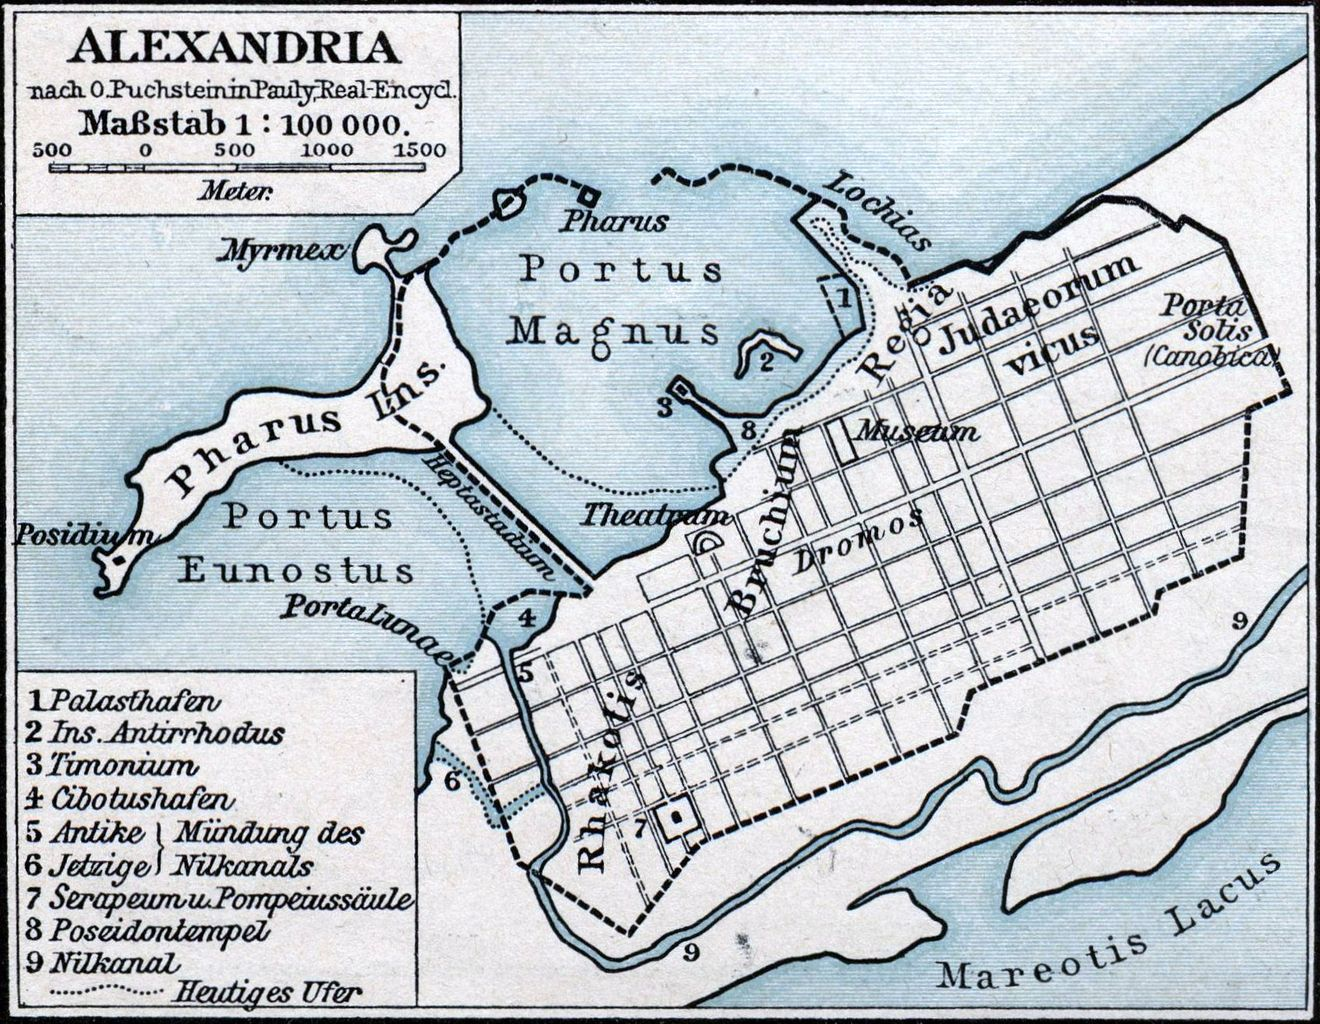
\includegraphics[width=8cm]{Mapa.jpg}
\end{center}
\caption{\label{fig:Mapa}
Mapa da antiga Alexandria (imagem extraída do atlas escolar de F. W. Putzgers)}   
\end{figure}

Embora detalhes biográficos sobre Euclides sejam
escassos, sua conexão com o Museu de Alexandria
reforça a imagem de um erudito imerso em um centro
de aprendizado dinâmico. O contraste entre a
durabilidade das ideias contidas nos \emph{Elementos} e a
efemeridade de construções físicas, como o Farol
de Alexandria, do qual não sobram nem ruínas,
apesar de ter resistido por séculos, já sublinha o
impacto perene da obra. Enquanto monumentos
materiais desapareceram, o sistema lógico e
dedutivo dos \emph{Elementos} continua a iluminar o
estudo da matemática, atestando a força das ideias
no transcorrer do tempo.

\section{Recepção}

A recepção inicial dos \emph{Elementos} no contexto da
matemática grega antiga não foi marcada por uma
aclamação universal imediata, mas por um processo
gradual de reconhecimento de sua importância.
Evidências históricas sugerem que a obra de
Euclides, embora seminal, enfrentou críticas e
debates em seus primeiros séculos. Um dos
primeiros registros de interação com \emph{Os Elementos}
vem de Apolônio, um matemático que viveu pouco
após Euclides. Nesta citação, tirada da obra
Cônicas (185 a.C.), Apolônio parece ter
questionado aspectos do tratamento dado por
Euclides a certos lugares geométricos em um 
trabalho infelizmente perdido:
\begin{quote} 
	E quando os descobrimos, percebemos que Euclides
	não havia feito a síntese do lugar geométrico em
	três e quatro linhas, mas apenas um fragmento
	acidental dele, e mesmo isso não foi feito com
	felicidade.
\cite{jones2005} 
\end{quote} 
Essa crítica inicial indica que \emph{Os Elementos}
não foi imediatamente aceito como uma obra-prima
incontestável, mas sim submetido ao escrutínio
acadêmico típico do período helenístico.

Outra menção a Euclides, dessa vez mais elogiosa,
aparece no diálogo \emph{De Oratore} de Cícero, escrito
em meados do primeiro século a.C. Numa 
crítica ao excesso de especialização nas 
artes e ciências, um dos interlocutores indaga:
\begin{quote}
	(\dots) Você supõe que a geometria sob Euclides e
	Arquimedes, a música sob Damão e Aristóxeno,
	a própria gramática quando Aristófanes e Calímaco
	trataram dela, eram tão divididas em partes
	que ninguém compreendia o sistema universal 
	de nenhuma dessas ciências, mas diferentes 
	pessoas selecionavam diferentes partes nas 
	quais pretendiam dedicar seu trabalho?
	(Cic. de Orat. 3.132)
\end{quote}


Posteriormente, por volta de 320 d.C., Papo de
Alexandria emerge como um defensor de Euclides,
respondendo às críticas de Apolônio e reforçando a
relevância da obra:
\begin{quote}
	Ele (Euclides) era extremamente justo e gentil
	com todos que eram capazes de ajudar a
	acrescentar algo à matemática... e nada
	ofensivo, um homem exato, mas não um fanfarrão
	--- como esse sujeito (Apolônio).
	\cite{jones2005}
\end{quote}
Esse diálogo acadêmico, separado por séculos,
reflete a continuidade do debate intelectual em
torno dos \emph{Elementos} e sua consolidação como
referência fundamental. Contudo, o comentário mais
significativo sobre a obra na antiguidade vem de
Proclo, por volta de 450 d.C., aproximadamente
sete séculos após a composição dos \emph{Elementos}. O
comentário de Proclo, focado especialmente no
Livro I, tornou-se um texto influente para as
gerações posteriores, moldando a compreensão da
obra de Euclides. \footnote{Acidentalmente, destacam-se os
desafios de preservar e interpretar um
\emph{corpus} matemático complexo em uma era com
recursos limitados para transmissão de
conhecimento, comparável à dificuldade de
interpretar hoje uma obra do século XIV com base
em fragmentos e comentários tardios.}

Proclo oferece uma perspectiva amplamente aceita
na antiguidade:
\begin{quote}
	Euclides, que não era muito mais jovem que
	Hermótimo e Filipo, compôs \emph{Elementos},
	ordenando muitos dos teoremas de Eudoxo,
	aperfeiçoando muitos dos que haviam sido
	trabalhados por Teeteto e fornecendo provas
	rigorosas de proposições que haviam sido
	demonstradas com menos rigor por seus
	antecessores.
	\cite{jones2005}
\end{quote}
Assim, Euclides não teria criado \emph{ex nihilo}
os teoremas apresentados nos \emph{Elementos}, mas agido
como um compilador e organizador do conhecimento
matemático de seus predecessores, como Eudoxo e
Teeteto, por exemplo. A inovação central de
Euclides, conforme enfatizado por Proclo, reside
na sistematização do conhecimento e na apresentação de
provas rigorosas dentro de uma estrutura dedutiva
coerente, ou seja, no método. 
%Essa abordagem
%metódica, que organizou teoremas preexistentes em
%um sistema unificado, constitui a
%contribuição mais duradoura dos \emph{Elementos},
%consolidando sua posição como um marco na história
%da matemática.

\section{Organização}

\emph{Os Elementos} constitui-se de uma coleção abrangente de
fatos matemáticos, na maior parte
geométricos ou descritos em termos 
geométricos, organizados em uma estrutura \emph{dedutiva}
na qual fatos mais complexos são \emph{demonstrados}
(explicados, justificados) através de fatos
mais simples.
Diferentemente
das tradições da Babilônia e do Egito, que se
concentravam em procedimentos práticos para
resolver problemas específicos, como cálculos de
áreas e volumes, a estrutura dos \emph{Elementos} prioriza a
demonstração de \emph{proposições} (os fatos
matemáticos) a partir de
\emph{definições}, \emph{postulados}, \emph{noções comuns}, 
que são os pontos de partida da investigação,
e de outras proposições previamente demonstradas. 

A obra abrange uma ampla
gama de fatos, desde fundamentos geométricos até
teoria dos números e geometria espacial, e está  
dividida em treze\footnote{Dois livros adicionais 
sobre geometria espacial, considerados 
apócrifos, aparecem em manuscritos antigos.} \emph{Livros}:
\begin{description}
	\item[Livro I:] Estabelece os fundamentos da geometria
		plana, abordando construções básicas, propriedades de
		triângulos, linhas paralelas e culminando na prova
		geométrica do Teorema de Pitágoras.
	\item[Livro II:] Explora a chamada ``álgebra
		geométrica'', utilizando figuras como quadrados e
		retângulos para demonstrar identidades algébricas,
		como as envolvendo o quadrado da soma e a diferença de
		quadrados, embora o termo ``álgebra geométrica'' seja
		debatido entre historiadores. 
		Este livro também introduz a razão áurea.
	\item[Livro III:] Focado em círculos, aborda
		propriedades de cordas, tangentes e ângulos inscritos,
		consolidando a compreensão geométrica de figuras
		circulares.
	\item[Livro IV:] Trata da inscrição e circunscrição de
		polígonos regulares (como triângulos equiláteros,
		quadrados, pentágonos e hexágonos) em círculos,
		utilizando apenas régua e compasso, reforçando
		técnicas de construção geométrica.
	\item[Livro V:] Apresenta a teoria da proporção de
		Eudoxo, uma conquista teórica notável que oferece um
		método rigoroso para lidar com grandezas
		incomensuráveis, como a razão entre a diagonal e o
		lado de um quadrado ($\sqrt{2}$). 
		Especula-se que essa teoria tenha surgido para
		resolver a chamada ``crise dos irracionais'' (embora seja
		discutível se essa ``crise'' realmente existiu),
		permitindo comparações de proporções sem atribuir
		valores numéricos.
	\item[Livro VI:] Aplica a teoria da proporção à
		similaridade de figuras, incluindo triângulos e
		polígonos, e reformula o Teorema de Pitágoras em
		termos de 
		figuras semelhantes em triângulos retângulos.
	\item[Livros VII, VIII e IX:] Deslocam o foco para a
		teoria dos números, tratada geometricamente, com
		números representados como segmentos de reta. O Livro
		VII introduz conceitos como divisibilidade, números
		primos e o algoritmo euclidiano para encontrar o
		máximo divisor comum. O Livro VIII explora progressões
		geométricas, enquanto o Livro IX inclui resultados
		fundamentais, como a prova da infinitude dos números
		primos e a construção de números perfeitos pares
		(iguais à soma de seus divisores próprios, como 6 e
		28), vinculados aos primos de Mersenne.
	\item[Livro X:] Considerado altamente complexo,
		classifica diferentes tipos de grandezas
		incomensuráveis, como retas irracionais relacionadas a
		raízes quadradas, demonstrando a profundidade técnica
		da obra.
	\item[Livros XI e XII:] Passam à geometria sólida,
		abordando linhas, planos, ângulos sólidos,
		paralelepípedos (Livro XI) e o cálculo de volumes de
		pirâmides, cones e esferas por meio do ``método da
		exaustão'', um precursor do cálculo integral (Livro
		XII).
	\item[Livro XIII:] Concentra-se na construção
		dos cinco sólidos platônicos (tetraedro, cubo,
		octaedro, dodecaedro e icosaedro). A escolha
		de concluir a obra com esses poliedros
		regulares, associados na filosofia platônica
		aos elementos fundamentais do cosmos, sugere
		possíveis influências platônicas na estrutura
		dos \emph{Elementos}, embora isso permaneça objeto de
		especulação acadêmica. 
\end{description}

No início de cada livro, são elencadas 
definições de termos que serão usados nas
demonstrações  subsequentes. Algumas das
definições encontradas  
no Livro I são, por exemplo:
\begin{description}
\item[Def.1] Um \emph{ponto} é aquilo que não possui partes.
\item[Def.2] Uma \emph{linha} é comprimento sem largura.
\item[Def.3] As \emph{extremidades} da linha são pontos.
\item[Def.4] \emph{Linha reta} é aquela que está 
posta igualmente entre suas extremidades.
\item[Def.10] Quando uma linha reta elevada sobre uma 
linha reta torna os ângulos adjacentes iguais entre si, 
cada um dos ângulos iguais é \emph{reto}, e a linha
reta sobre o outro é chamada \emph{perpendicular}
àquela em que está.
\item[Def.15] Um \emph{círculo} é uma figura plana 
contida por uma linha tal que todas as linhas retas
que caem sobre ele a partir de um ponto entre aqueles
que estão dentro da figura são iguais entre si.
\end{description}

%A estrutura sistemática dos \emph{Elementos}, com sua progressão
%lógica e abrangência, não apenas consolida o conhecimento
%matemático da época, mas também estabelece um paradigma de
%rigor dedutivo que continua a influenciar a matemática
%contemporânea. A inclusão de tópicos como a infinitude dos
%números primos e a questão ainda não resolvida dos números
%perfeitos ímpares demonstra a profundidade e a relevância
%duradoura da obra.
Além disso, no Livro I são elencados cinco \emph{postulados}:
\begin{enumerate}
\item    Fique postulado traçar uma reta a partir de todo ponto até todo ponto.
\item    Também prolongar uma reta limitada, continuamente, sobre uma reta.
\item    E, com todo centro e distância, descrever um círculo.
\item     E serem iguais entre si todos os ângulos retos.
\item    E, caso uma reta, caindo sobre duas retas, faça os ângulos interiores e do mesmo lado menores do que dois retos, sendo prolongadas as duas retas, ilimitadamente, encontrarem-se no lado do qual estão os menores do que dois retos.
\end{enumerate}
e cinco \emph{noções comuns}:
\begin{enumerate}
    \item 
  Coisas iguais a uma coisa são iguais entre si.
\item  Se a coisas iguais foram somadas coisas iguais, as somas também serão iguais.
\item  Se de coisas iguais forem subtraídas coisas iguais, os restos também serão iguais.
%\item  E se coisas iguais forem somadas a coisas desiguais, as somas serão desiguais.
%\item  E coisas iguais ao dobro da mesma coisa são iguais entre si. 
%\item  E as metades da mesma coisa são iguais entre si. 
\item  Coisas que coincidem entre si são iguais. 
\item O todo é maior que suas partes.
\end{enumerate}

Postulados e noções comuns são normalmente
interpretados como fatos tão intuitivos 
que não precisam de demonstração e que 
baseiam, portanto, toda investigação subsequente. 
Mais adiante, outra interpretação será 
aventada. Os postulados tratam de fatos 
puramente geométricos, enquanto as noções
comuns estão relacionadas a fatos gerais 
que se aplicam possivelmente a outras ciências. 



\section{Estrutura de uma Demonstração}

A análise da estrutura das provas nos \emph{Elementos},
conforme delineada por Proclo no século V d.C.,
oferece uma visão detalhada da abordagem
metodológica de Euclides. Proclo identificou seis
componentes distintos em uma proposição típica da
obra, refletindo a organização lógica e
sistemática que caracteriza o texto. Esses
componentes são (com os nomes correspondentes
em grego entre parêntesis): 
\begin{description}
	\item[Enunciação  (\emph{protasis}):] A declaração inicial do que
		será provado ou construído, apresentando a
		proposição de forma geral.
	\item[Exposição (\emph{ekthesis}):] A definição de um \emph{diagrama} 
	 específico, com
		a atribuição de rótulos aos elementos relevantes, como
		pontos e linhas.
	\item[Determinação  (\emph{diorismos}):] A reafirmação do objetivo da proposição, agora
		em termos da figura específica introduzida na exposição.
	\item[Construção (\emph{kataskeue}):] A adição de novos elementos geométricos,
	  como pontos, linhas
		ou círculos, necessários para desenvolver a prova.
	\item[Demonstração (\emph{apodeixis}):] A descrição passo a passo 
		do argumento que
		estabelece a veracidade da proposição, referindo-se a
		definições, 
		postulados, noções comuns e resultados anteriores.
	\item[Conclusão (\emph{sumperasma}):] A reafirmação da proposição
original como provada, encerrando a demonstração.
\end{description}
Essa estrutura é exemplificada na primeira
proposição do Livro I, que propõe a construção de
um triângulo equilátero a partir de um segmento de
reta dado:
\begin{description}
	\item[Enunciação] Sobre uma linha reta finita,
	 construir um triângulo equilátero. 
	\item[Exposição] Seja $AB$ a linha reta finita dada.
	\begin{center}
			\begin{tikzpicture}[scale=0.5]  
\tkzDefPoint(-2,0){A}    
\tkzDefPoint(2,0){B}
\tkzDrawCircle[line width=1.25pt](A,B)
\tkzDrawCircle[line width=1.25pt](B,A)
\tkzDefTriangle[equilateral](A,B)
\tkzGetPoint{C}
\tkzDrawPolygons(A,B,C)
\tkzDefPointOnLine[pos=2](A,B)\tkzGetPoint{E}
\tkzDefPointOnLine[pos=2](B,A)\tkzGetPoint{D}
\tkzLabelPoints[left](A)
\tkzLabelPoints[right](B)
\tkzLabelPoints[left](D)
\tkzLabelPoints[right](E)
\tkzLabelPoints[above](C)
\tkzDrawPoints(A,B,C)
\end{tikzpicture}
	\end{center}

	\item[Determinação] Assim, deve-se construir um
	triângulo equilátero sobre $AB$.
	\item[Construção] Com o centro $A$ e com distância $AB$
	 se descreva (Post. 3) o círculo $BCD$; e com o centro $B$
	e com distância $BA$ se descreva o círculo $ACE$.
	 Do ponto $C$, onde os círculos se cortam reciprocamente,
	se tracem (Post. 1) para os pontos $A$ e $B$ as retas $CA$ e $CB$.
	\item[Demonstração] Sendo o ponto $A$ o centro do círculo 
	$BCD$, $AC$ é igual a $AB$ (Def. 15). E sendo o ponto $B$
	 o centro do círculo $CAE$, $BC$ é igual a $BA$.
	  Mas foi provado que $CA$ é igual a $AB$. Logo tanto $CA$
		 como $CB$ são iguais a $AB$. Mas as coisas que são iguais
		  a uma terceira são iguais entre si (Noção Comum 1).
		Logo $CA$ é igual a $CB$.
		Logo as três retas $CA$, $AB$ e $BC$ são iguais.   
\item[Conclusão]  Por consequência, o triangulo $ABC$,
 construído sobre a linha reta finita dada $AB$, é equilátero.
	\end{description}

Esse mesmo esquema é seguido, com poucas exceções, ao longo
dos treze livros. Euclides distingue dois tipos de
proposições: \emph{problemas}, que têm o objetivo 
de demonstrar a possibilidade de construir certos
objetos, como o triângulo equilátero no caso acima,
e \emph{teoremas}, que visam estabelecer certos
fatos, como por exemplo a Proposição I.47 (o Teorema
de Pitágoras). A estrutura da demonstração é a 
mesma em ambos os casos, mas há pequenas variações
de linguagem. Por exemplo, emprega-se o modo
imperativo \footnote{em grego, normalmente traduzido
para o infinitivo em português.} 
para  na enunciação de problemas 
(``Construa um triângulo\dots'' ou ``Construir um
triângulo\dots'') e o modo
indicativo nos teoremas (``Em triângulos retângulos,
o quadrado do lado que subtende o ângulo reto é
 igual aos quadrados dos lados que contêm o ângulo reto'').
 Também os problemas terminam com a expressão
 ``o que era preciso fazer'' 
 (\emph{quod erat faciendum}, em latim, abreviado por 
 QEF), enquanto os 
 teoremas se encerram com ``o que era preciso mostrar''
 (\emph{quod erat demonstrandum}, abreviado por 
 QED).

Há uma extensa literatura sobre
as origens, motivações e propósitos de 
tal estrutura demonstrativa, com visões
por vezes contraditórias. Algumas pontos,
entretanto, parecem certos:
\begin{itemize}
\item A redundância das hipóteses e teses e o uso
de uma linguagem formulaica, repetitiva,
facilita a memorização das proposições.
\item O diagrama que aparece na exposição tem
uma função essencial, sendo uma característica 
inconfundível dos \emph{Elementos}, 
mesmo que a necessidade
de figuras para a demonstração de fatos 
gerais tenha sido questionada desde a antiguidade,
pois elas representam apenas casos particulares 
das proposições e ainda são desenhadas de maneira
necessariamente imperfeita.
\item A etapa de construção isola o aspecto
criativo do argumento, na medida em que introduz
novos objetos que serão utilizados
decisivamente na etapa de demonstração.
\end{itemize} 

% Nessa prova, Euclides constrói dois
% círculos, cada um centrado em uma extremidade do
% segmento, com o comprimento do segmento como raio,
% e assume que esses círculos se intersectam para
% formar o terceiro vértice do triângulo. Contudo,
% sob a perspectiva de sistemas matemáticos
% modernos, essa suposição apresenta uma lacuna
% lógica, pois a interseção dos círculos exigiria um
% axioma de continuidade para ser rigorosamente
% garantida. Essa aparente falha reflete a questão
% do anacronismo, pois os padrões de rigor formal
% contemporâneos não se aplicavam ao contexto
% intelectual de Euclides. No entanto, a
% interpretação dialética proposta por Árpád Szabó
% oferece uma leitura alternativa. Se \emph{Os Elementos}
% é visto como enraizado na tradição dialética
% grega, na qual postulados e definições servem como
% pontos de partida consensuais para a argumentação,
% a suposição implícita da interseção dos círculos
% pode não ter sido percebida como uma falha. Nesse
% contexto, os participantes do discurso geométrico,
% ao aceitarem os postulados de construção (como a
% possibilidade de desenhar círculos com régua e
% compasso), poderiam considerar a interseção
% visualmente evidente como suficiente para a
% progressão do argumento. Assim, a estrutura das
% provas de Euclides reflete menos uma tentativa de
% atingir um rigor lógico absoluto e mais um esforço
% para estabelecer um discurso geométrico coerente
% dentro de um quadro dialético acordado.

% Essa perspectiva sublinha a importância de compreender os
% Elementos em seu contexto histórico, evitando julgamentos
% anacrônicos baseados em critérios modernos. A análise de
% Proclo, ao destacar a organização sistemática das
% proposições, reforça a relevância da obra como um marco na
% história do pensamento matemático, cuja influência persiste
% pela sua capacidade de estruturar argumentos de maneira
% lógica e acessível.

\section{Anacronismo}

A interpretação dos \emph{Elementos} pode ser obscurecida
pelo \emph{anacronismo}, isto é, pela tendência de
julgá-los com base nos padrões modernos de lógica
matemática e sistemas axiomáticos, desenvolvidos
principalmente nos séculos XIX e XX \footnote{
O prof. Papini deu sua visão sobre este 
desenvolvimento na edição anterior desta revista
\cite{Papini2024} (N. do E.).}. Sob essa
perspectiva contemporânea, \emph{Os Elementos} apresenta
aparentes lacunas e imperfeições. Por exemplo, as definições de
Euclides, como a de um ponto como ``aquilo que não
tem parte'' ou de uma reta como ``comprimento sem
largura'', carecem do rigor exigido em sistemas
formais modernos, nos quais tais termos são
frequentemente tratados como conceitos primitivos
indefinidos. Além disso, análises contemporâneas
revelam que Euclides ocasionalmente se apoia em
suposições implícitas não declaradas em seus
postulados ou noções comuns, muitas vezes 
tiradas das figuras, como propriedades de
continuidade ou a ordem de pontos em uma reta. 
Por exemplo, o que garante que os dois círculos 
traçados na proposição detalhada na seção anterior 
de fato se intersectam?

Essa crítica, no entanto, levanta uma questão fundamental:
\emph{estaria Euclides sendo descuidado pelos padrões modernos, ou
estaria ele operando dentro de um paradigma intelectual
distinto?}

Uma interpretação alternativa, proposta pelo
estudioso húngaro Árpád Szabó em \cite{szabo1967},
sugere que \emph{Os Elementos} tem
raízes menos na lógica formal aristotélica, ainda em
desenvolvimento na época, e mais na tradição grega da 
\emph{dialética}, caracterizada pela argumentação estruturada entre
perspectivas opostas, como no método socrático. Szabó
argumenta que a terminologia de Euclides reflete essa
abordagem. Por exemplo, a palavra grega \emph{hypothesis}
(hipótese), usada por Euclides, não denotaria apenas uma
suposição lógica, mas uma proposição consensual estabelecida
como ponto de partida para um debate: 
\begin{quote}
	A palavra grega \emph{hipótese} deriva da preposição
	\emph{hypo} (sob, abaixo de) e do verbo \emph{tithesthai}
	(por, colocar) e significa, de fato, aquilo que
	duas pessoas engajadas em uma conversa, dois 
	adversários em um debate, mutuamente concordam como
	base e ponto de partida de seu debate. (\dots)
	O primeiro tipo de hipótese são as \emph{definições},
	as quais para os gregos eram circunscrições, dadas sem
	prova, de conceitos (noções) usadas em matemática.
	\cite{szabo1967}
\end{quote}
Assim, definições como
a de ponto ou reta não visariam ao rigor lógico absoluto, mas
sim delimitar os termos da discussão, estabelecendo um
acordo sobre os conceitos fundamentais a serem explorados.

Na sequência, Szabó indaga:
\begin{quote}
	Mas o que acontece se os disputantes não podem
	encontrar asserções mutuamente aceitáveis
	de onde começar? (\dots) Neste caso, não há 
	base mútua aceitável para a discussão 
	subsequente; e um dos adversários não pode começar
	de uma `hipótese' mas apenas de uma asserção
	mais forte tomada como ponto de partida \emph{por ele}
	--- de um `\emph{axioma}'. A palavra grega
	`axioma' originalmente significando `petição' 
	(pedido, requerimento, exigência); um adversário
	requer que o outro aceite sua asserção como 
	ponto de partida do debate.
\end{quote}
A palavra grega para postulado é \emph{aitemata},
significando literalmente `demanda', `pedido',
sendo portanto quase um sinônimo de `axioma'.
Mas se postulados são asserções mais fortes que 
um adversário demanda do outro, \emph{o que haveria
de tão forte assim nos postulados de Euclides?
Não é intuitivamente óbvio que seja possível
traçar uma linha reta entre dois pontos ou
um círculo com centro e raio dados?} 

\begin{figure}[htb!]
\begin{center}
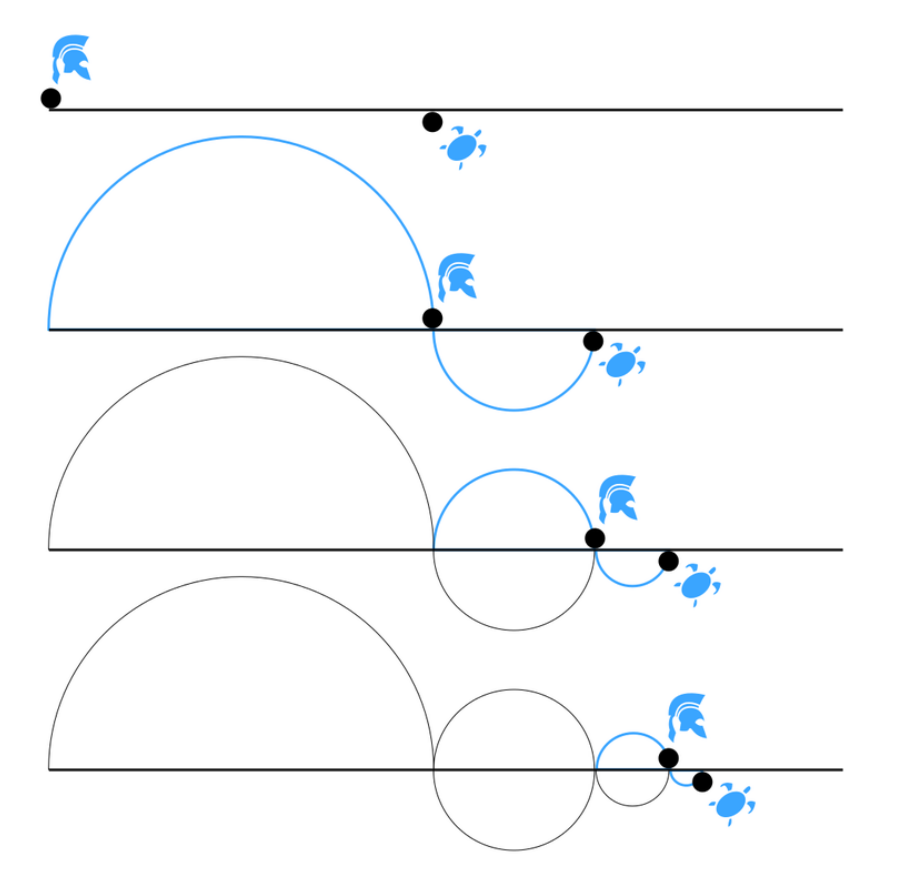
\includegraphics[width=9cm]{Aquiles.png}
\end{center}
\caption{\label{fig:Aquiles}
Para alcançar a tartaruga, Aquiles precisa primeiro 
chegar ao ponto onde a tartaruga estava. 
No entanto, nesse ponto, a tartaruga já avançou 
para uma nova posição. 
Para alcançar essa nova posição, Aquiles precisa 
cobrir mais uma distância, e assim por diante,
de modo que ele nunca ultrapassará a tartaruga.
(Fonte: Wikipedia)}   
\end{figure}

Para Zenão de Eleia e outros filósofos
da escola eleática, os quais questionavam a coerência
de conceitos como movimento e divisibilidade
através de vários paradoxos engenhosos, como
o paradoxo de ``Aquiles e a Tartaruga'' (Fig. \ref{fig:Aquiles}),
a resposta poderia ser: ``Não, não é óbvio, 
e mesmo que o fosse, tratando a matemática de
verdades eternas, demonstrações não deveriam
invocar a ideia de movimento''. 

Assim, os três primeiros postulados seriam
exigências para aceitar a possibilidade de construções
geométricas fundamentais, utilizando ferramentas como régua
e compasso:
\begin{quote}
	A única maneira de tornar as construções 
	geométricas teoricamente possíveis
	é admitindo ao menos três tipos de movimentos
	que são indispensáveis para a produção das
	formas geométricas mais simples (linhas retas,
	círculos e seus pontos de interseção).(\dots)
	Eles são realmente \emph{demandas} (\emph{aitemata},
	 postulados) e não \emph{acordos} (\emph{homologemata}),
	 pois eles postulam movimento [que é inaceitável
	 para os Eleatas].\cite{szabo1978}	
\end{quote}
Em resumo, os postulados funcionam como
condições para viabilizar o discurso geométrico,
e não como verdades intuitivamente óbvias.

As noções comuns (\emph{koinai ennoiai}), por sua vez, abordam
princípios gerais de igualdade e magnitude, que 
também poderiam ser 
questionadas no contexto filosófico da
época: 
\begin{quote}
	Ao contrário, todas as propriedades afirmadas 
	da relação [de igualdade] deveriam ser vistas
	(ao menos para os Eleatas) como autocontraditórias.
	Não é nada evidente como duas coisas distintas
	(i.e. coisas que não são as mesmas) podem
	jamais ser `\emph{iguais uma a outra}'.(\dots)
	Os Eleatas estavam dispostos a conceder apenas 
	que uma coisa possa ser \emph{igual a si mesma},
	não que ela pudesse igualar \emph{outra coisa}.
	\cite{szabo1978}
\end{quote}
Ou seja, filósofos eleáticos poderiam questionar a igualdade de
entidades distintas ou a relação entre o todo e suas partes,
especialmente considerando paradoxos envolvendo o infinito.
Na matemática moderna, por exemplo, conjuntos infinitos
desafiam a noção de que o todo é maior que a parte, como
demonstrado pela correspondência biunívoca entre um conjunto
infinito e certos subconjuntos próprios. Assim, as noções
comuns de Euclides seriam demandas baseadas na
experiência comum com grandezas finitas, aceitas para
permitir o discurso matemático.

Mais recentemente, e numa direção semelhante, 
Novaes afirma em \emph{The Dialogical Roots of Deduction}
(``As Raízes Dialógicas da Dedução'') \cite{Novaes2020}
que
\begin{quote}
	Podemos assim dizer que a demonstração [em Euclides] representa
	um `diálogo' entre o autor do texto e seus leitores, os 
	quais são instruídos a levar a cabo certos procedimentos.
\end{quote}
Ou seja, à medida que Euclides, o ``provador''
interessado em demonstrar uma proposição, vai descrevendo as
etapas da construção e da demonstração, e o leitor,
talvez até inicialmente ``cético'', 
as vai reconstruindo mentalmente (ou mesmo fisicamente
com régua e compasso), com a ajuda do diagrama,
estabelece-se um diálogo ativo,
bem ao estilo grego, produzindo um efeito persuasivo bem maior
do que a mera leitura de um argumento puramente textual. 
Nesse processo dialógico, a existência do 
ponto de interseção entre os círculos traçados
na Proposição 1, por exemplo, fica evidente,
não sendo um problema de fato. 

As objeções quanto ao uso de figuras em 
demonstrações também foram desafiadas através
de uma análise detalhada do filósofo 
Kenneth Manders em ``The Euclidean Diagram''
(O Diagrama Euclidiano) \cite{Manders95}. Resumindo um
longo argumento,
Manders inicialmente lembra que, embora 
conclusões errôneas possam ser retiradas
de figuras, isso muito raramente foi um problema
na prática de dois mil anos de
geometria euclidiana, o que sugere um 
uso \emph{controlado} das figuras. A seguir,
ele faz uma distinção entre propriedades
que ele denominou \emph{co-exatas}, 
tais como incidência entre retas e ordem entre
pontos em uma reta, que não variam caso 
os dados da figura sejam ligeiramente perturbados,
e as propriedades \emph{exatas}, como 
medidas de segmentos e perpendicularidade, que variam.  
Como bem resume Santos de Jesus \cite{deJesus2023},
\begin{quote}
O principal erro nas objeções às demonstrações
euclidianas foi assumir que
qualquer afirmação era justificada pelo diagrama.
Euclides não procede assim. Nos
Elementos, uma propriedade exata nunca é extraída
dos diagramas. Já as propriedades
topológicas, as co-exatas, não dependem da precisão
com que os diagramas são desenhados,
senão do controle sobre a manipulação da figura,
controle este que depende da estabilidade da
prática matemática.
\end{quote}
Após a crítica de Manders, outros pesquisadores
propuseram maneiras de incorporar formalmente
diagramas nos esquemas dedutivos \cite{mumma2006, avigad2009}. 

Essas interpretações reconfiguram
 \emph{Os Elementos} como
uma obra menos voltada para a construção de um sistema
lógico atemporal e mais focada em estabelecer um argumento
estruturado com base em pontos de partida consensuais. Essa
perspectiva destaca a natureza contextual da obra, enraizada
nas práticas intelectuais de sua época, e oferece uma lente
alternativa para compreender sua estrutura e propósito.

\section{Edições}

% O impacto dos \emph{Elementos} de Euclides transcende seu contexto
% original, tendo influenciado profundamente o desenvolvimento
% da matemática através de sua transmissão, tradução e
% adaptação ao longo dos séculos. Após sua composição, a obra
% foi objeto de estudo e comentário contínuos, garantindo sua
% preservação e relevância em diferentes culturas e épocas.

A história das edições dos \emph{Elementos}
é muito complexa (como detalhada em \cite{derisi2016} 
e \cite{Wardhaugh2021}), mas um breve resumo
é necessário para se entender o alcance
do \emph{Farol de Euclides}.
Na Antiguidade Tardia, uma edição comentada por Teon de
Alexandria, cuja filha Hipátia dá nome a esta revista,
tornou-se amplamente
influente. Esse momento coincide com
o declínio de Alexandria e a ascenção
de Constantinopla (Bizâncio)
como centro do mundo helenístico. Uma 
lindo exemplar bizantino de 888 d.C., 
um livro em pergaminho que pertenceu
a Aretas de Patras, é o mais antigo
manuscrito grego dos \emph{Elementos}
com uma data estampada na capa.
Uma tradução do grego para o árabe
foi realizada por al-Hajjaj no século IX.
Estudiosos do mundo islâmico não apenas
preservaram o texto, mas também o expandiram com novos
comentários e interpretações, enriquecendo seu conteúdo. Nos
séculos XI e XII, a transmissão dos \emph{Elementos} para a Europa
Ocidental foi mediada por tradutores como Adelardo de Bath,
que, viajando para regiões como Espanha e Sicília,
traduziram versões árabes para o latim. Esse processo
reintroduziu a obra no contexto europeu, onde ela se
tornaria uma pedra angular do pensamento matemático
medieval.

\begin{figure}[htb!]
\begin{center}
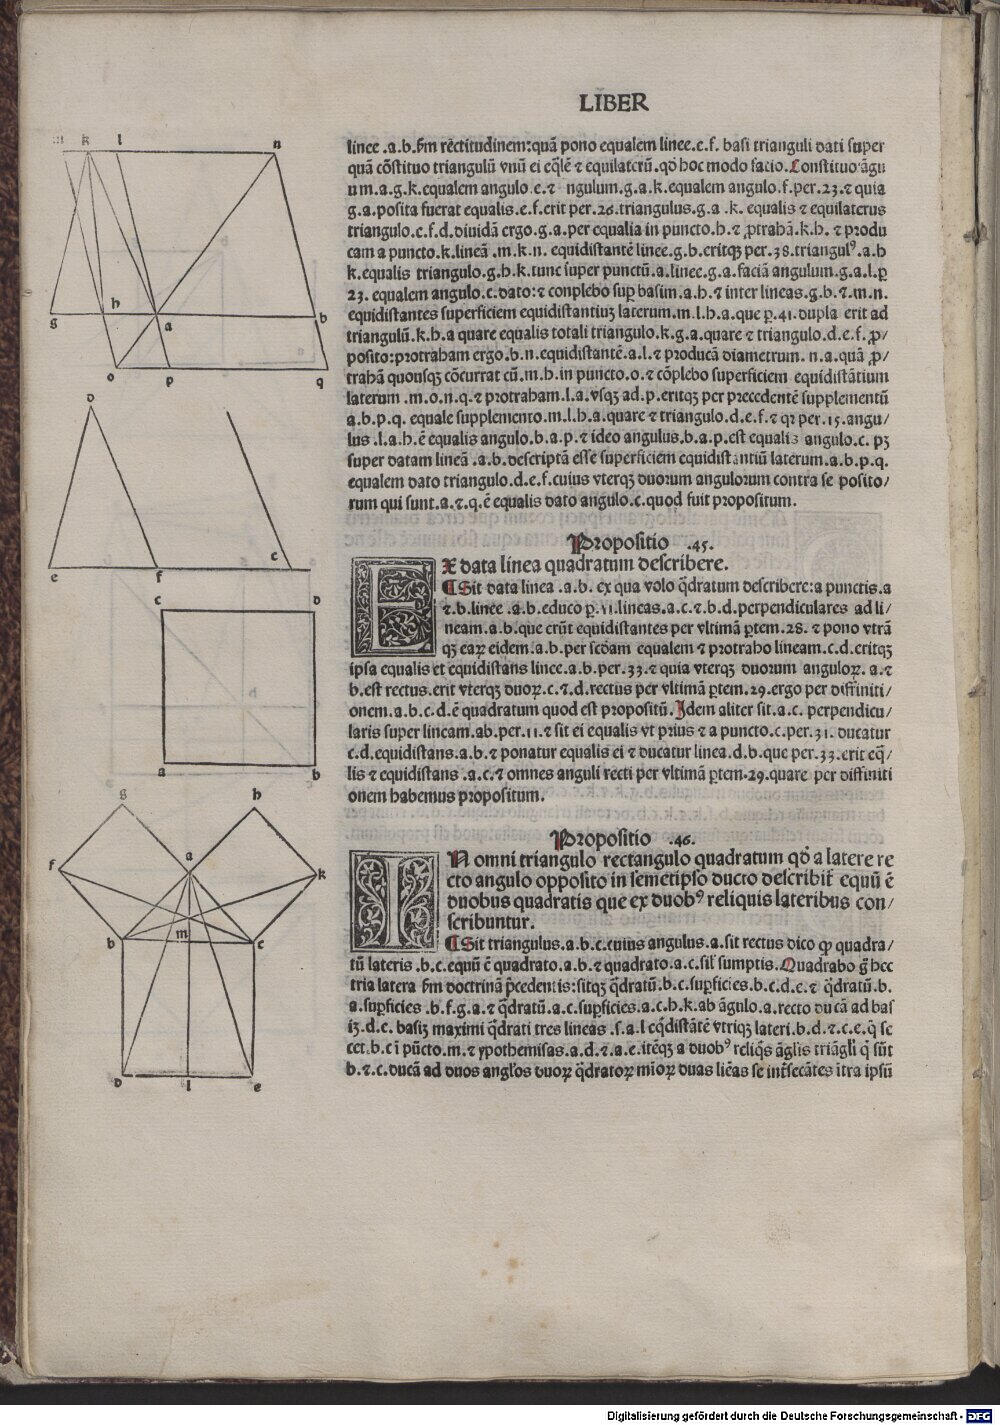
\includegraphics[width=8cm]{princeps.jpg}
\end{center}
\caption{\label{fig:Princeps}
Em 25 de maio de 1482, o impressor Erhard Ratdolt,
de Veneza, lançou a primeira edição impressa
 (\emph{editio princeps}) dos Elementos de Euclides ---
 \emph{Praeclarissimus liber elementorum Euclidis in artem geometriae}.
  O texto de Ratdolt foi baseado em uma tradução do 
	árabe para o latim, presumivelmente feita por 
	Abelardo de Bath no século XII, editada e anotada 
	por Giovanni Compano (Campanus de Novara) no 
	século XIII. A primeira edição impressa de Euclides 
	foi o primeiro livro substancial a conter figuras 
	geométricas, das quais incluía mais de 400.
(Fonte: \emph{Bayerische Staatsbibliothek})}   
\end{figure}
A invenção da imprensa no século XV revolucionou a
disseminação dos \emph{Elementos}. A primeira edição impressa,
baseada numa manuscrito 
anterior composto por Campano de Novara, 
foi publicada por Ratdolt  em Veneza em 1482, 
tornando a 
obra significativamente mais acessível
(Fig. \ref{fig:Princeps}). Seguiram-se inúmeras
edições, incluindo versões baseadas em manuscritos gregos
redescobertos, como a de Simon Grynaeus de 1533,
e traduções influentes em línguas locais, como italiano
(Tartaglia, 1543), alemão (Xylander, 1562), 
francês (Forcadel, 1564), inglês (Billingsley, 1570),
espanhol (Zamorano, 1576) e holandês (Dou, 1606). No
final do século XVI, o matemático jesuíta Christopher
Clavius produziu uma edição em latim amplamente
utilizada, conhecida por seus extensos comentários.
No século XVII, a edição de Pierre Hérigone (1634)
introduziu símbolos matemáticos modernos, como o
símbolo $\perp$ para denotar perpendicularidade,
refletindo um esforço para
alinhar a obra com as convenções emergentes da matemática.
A partir daí, surgiram outras edições apenas
inspiradas pelos \emph{Elementos}, mas 
com axiomas e demonstrações diferentes,
como a influente
\emph{Éléments de géométrie avec des notes} (1794)
 de Legendre, cuja tradução para o português foi
 o primeiro livro de matemática impresso no Brasil 
 (1809).


No começo do século XIX, François Peyrard, trabalhando
com todos os manuscritos gregos disponíveis, inclusive
o famoso \emph{manuscrito 190} da biblioteca do 
Vaticano (o qual fora ``tomado de empréstimo'' 
pelas tropas napoleônicos durante a invasão da
Itália), compôs uma versão dos \emph{Elementos}
mais próxima do original, sem os acréscimos 
feitos desde o tempo de Teon. Posteriormente, 
por volta de 1880, 
o filólogo dinamarquês Heiberg continuou o trabalho
de Peyrard, produzindo a versão mais aceita
atualmente.

Muitas dessas edições buscavam ``aperfeiçoar'' 
\emph{Os Elementos}, adicionando-se novos 
postulados e novas definições, alterando-se a 
ordem, o número e a redação de algumas proposições,
tudo isso com o objetivo de se preencher as ``lacunas''
lógicas que eram percebidas, uma vez que 
o contexto cultural e filosófico que 
engendrou a obra já havia desaparecido.
De Risi \cite{derisi2016} realizou o trabalho
hercúleo de identificar os axiomas usados 
em cada uma das centenas de edições conhecidas
no ocidente num período de quase mil anos,
do manuscrito 190 até o começo do século XIX.

É necessário dizer, entretanto, que  
o entusiasmo gerado por essas edições
entre os eruditos 
não era compartilhado por gerações de
estudantes que eram obrigados a estudar
geometria \emph{à maneira de Euclides},
decorando enfadonhos teoremas, sem 
a motivação adequada e privados
daqueles elementos de \emph{performance},
diálogo e debate que caracterizavam o
método grego. 
O matemático Sylvester chegou a afirmar 
que 
\begin{quote}
Eu deveria me alegrar em ver (\dots) 
Euclides honrosamente arquivado ou enterrado 
``em lugar fundo, jamais tocado por nenhuma sonda''
fora do alcance dos estudantes; \cite[p. 286]{Wardhaugh2021}
\end{quote}

\begin{figure}[htb!]
\begin{center}
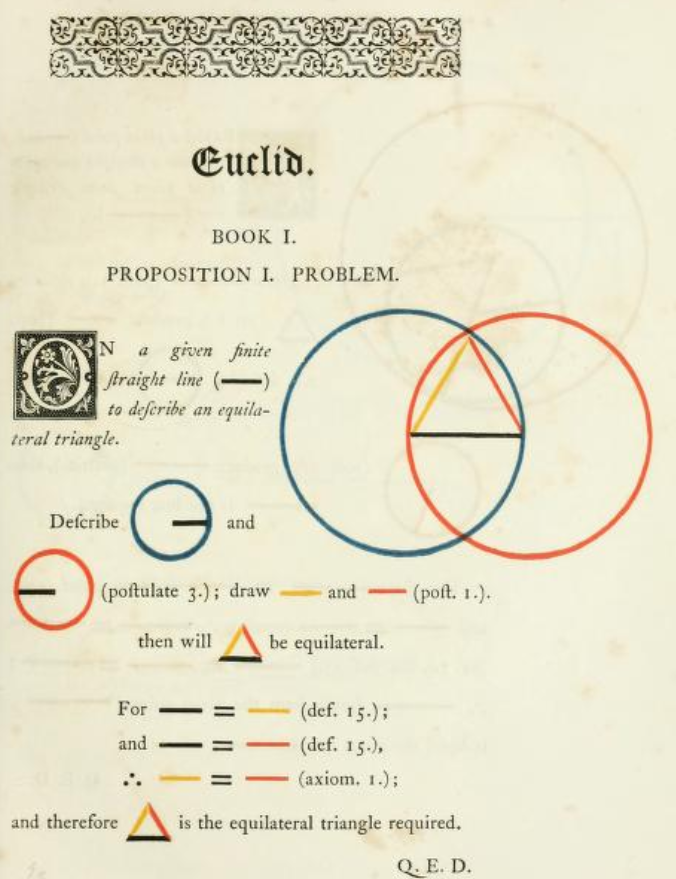
\includegraphics[width=8cm]{byrne.png}
\end{center}
\caption{\label{fig:Byrne}
Demonstração da Proposição I.1 na edição de Oliver Byrne.
(Fonte: Getty Research Institute)}   
\end{figure}

Talvez a necessidade de tornar o estudo dos 
\emph{Elementos} menos árido tenha levado
Oliver Byrne a editar sua versão em 1847 (Fig. \ref{fig:Byrne}), 
celebrada pela abordagem visual inovadora. Byrne
substituiu as tradicionais letras por diagramas e símbolos
codificados por cores para representar ângulos e retas nas
demonstrações, criando uma obra de grande apelo estético. Embora
não tenha alcançado sucesso comercial em sua época, essa
edição foi redescoberta recentemente por \emph{designers} e
bibliófilos, que a valorizam por sua singularidade visual e
valor artístico.


\section{Descartes}

Uma transformação significativa no pensamento geo\-métrico
ocorreu com a publicação de \emph{La Géométrie} por René Descartes
em 1637, que introduziu a \emph{geometria analítica}.
Ao utilizar
coordenadas e álgebra para resolver problemas geométricos,
Descartes ofereceu uma alternativa poderosa aos métodos
sintéticos de Euclides. Embora não tenha substituído
imediatamente a abordagem euclidiana, a geometria analítica
proporcionou uma nova ferramenta conceitual, expandindo as
possibilidades de análise geométrica e marcando uma
transição para paradigmas matemáticos modernos.
Segundo Thomsen \cite{Thomsen33},
\begin{quote}
    Enquanto antes de Descartes cada teorema exigia 
		para sua prova alguma ideia nova, algum acaso feliz, 
		como por exemplo o desenho de algumas linhas 
		peculiares na figura, a geometria analítica 
		fornece de uma vez por todas um meio infalível 
		de completar a prova em cada caso em um número 
		finito de etapas, apenas por diligência e rotina.
\end{quote}

Não seria exagero ombrear Euclides e Descartes na
história da matemática e das ideias em geral, tanto
é assim que seus nomes se tornaram adjetivos
de uso comum: euclidiano e cartesiano. Mas 
demorou um tempo para esse reconhecimento. 
Por exemplo, o filósofo Spinoza, inicialmente
influenciado por Descartes, descreveu a 
filosofia cartesiana usando a mesma 
estrutura dedutiva euclidiana
em seu livro \emph{Renati Descartes principia philosophiae,
 more geometrico demonstrata} (1663)! Posteriormente,
 Spinoza empregaria de novo o método euclidiano em 
 sua obra máxima, \emph{A Ética demonstrada à
  maneira dos geômetras} (1677).

Outro exemplo do peso do legado 
euclidiano é mais uma obra emblemática:
\emph{Princípios Matemáticos da Filosofia Natural} (1687),
de Isaac Newton. Newton era bem versado
tanto na tradição euclidiana, quanto na então
recente geometria cartesiana, tendo já 
desenvolvido seu cálculo na forma analítica
de Descartes, porém, ainda assim, talvez 
para facilitar a divulgação (ou para dificultar,
Newton era um sujeito esquivo), ele expôs seu
sistema numa linguagem aparentemente euclidiana,
na qual o cálculo se ocultava em expressões 
como ``razões finais'' de ``quantidades evanescentes''. 

Hoje em dia, essas duas maneiras de
abordar a geometria são vistas pela
maioria dos matemáticos como 
absolutamente complementares. 
Mas ainda há aqueles que veem uma
primazia dos métodos geométricos 
mais puros, como pode-se notar 
nesta citação de Michael Atiyah:
\begin{quote}
    Álgebra é a oferta feita pelo diabo ao matemático. 
		O diabo diz: ``Eu lhe darei esta máquina poderosa, 
		e ela responderá a qualquer pergunta que você quiser. 
		Tudo o que você precisa fazer é me dar sua alma: 
		desista da geometria e você terá esta máquina maravilhosa.''
		\dots o perigo para a nossa alma está aí, porque quando 
		você passa para o cálculo algébrico, essencialmente 
		você para de pensar: você para de pensar geometricamente, 
		você para de pensar no significado. \cite[p. xvii]{Needham2021}
\end{quote}

\section{Geometrias Não-Euclidianas}

O quinto postulado de Euclides, conhecido como o postulado
das paralelas, desempenhou um papel central na história da
matemática, desencadeando um dos debates mais profundos e
transformadores da disciplina. Durante séculos, matemáticos
buscaram demonstrar que esse postulado, que estabelece que,
dada uma reta e um ponto fora dela, existe exatamente uma
reta paralela à primeira passando por esse ponto, poderia
ser derivado dos outros quatro postulados. A percepção de
que o quinto postulado parecia menos intuitivo levou a
tentativas persistentes de provar sua dependência, sob a
suposição de que ele não era verdadeiramente independente.
Apesar desses esforços, nenhuma demonstração bem-sucedida
foi alcançada.

\begin{figure}[htb!]
\begin{center}
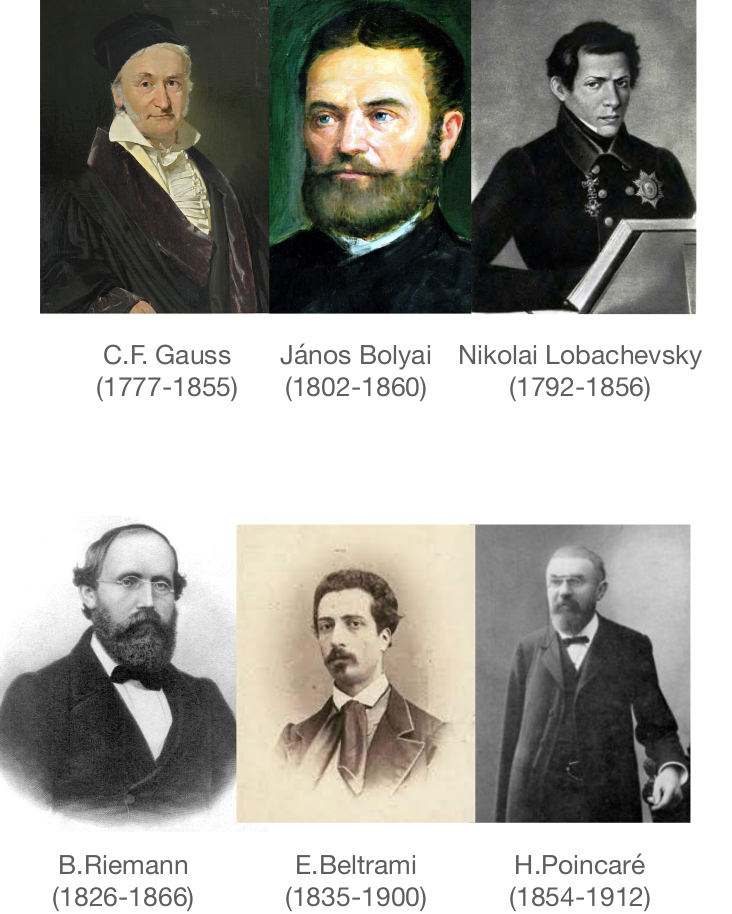
\includegraphics[width=8cm]{pioneiros.png}
\end{center}
\caption{\label{fig:Pioneiros}
Galeria de matemáticos pioneiros na 
exploração das geometrias não-euclidianas. 
(Fonte: Wikipedia)}   
\end{figure}

No início do século XIX, uma mudança paradigmática ocorreu
quando matemáticos como Carl Friedrich Gauss, János Bolyai e
Nikolai Lobachevsky, trabalhando de forma independente,
começaram a explorar as implicações de rejeitar o quinto
postulado (Fig. \ref{fig:Pioneiros}). Eles desenvolveram geometrias não-euclidianas,
nas quais o postulado das paralelas não se aplica, revelando
a possibilidade de sistemas geométricos consistentes que
descrevem espaços curvos, como os hiperbólicos e elípticos.
Posteriormente, no mesmo século, Bernhard Riemann
generalizou ainda mais essas ideias, estabelecendo os
fundamentos da geometria diferencial. Modelos formais
desenvolvidos por Eugenio Beltrami e Henri Poincaré
demonstraram que essas geometrias não-euclidianas eram tão
logicamente robustas quanto a geometria euclidiana, que
descreve o espaço plano. Essa descoberta revolucionou não
apenas a matemática, mas também a física, fornecendo
ferramentas conceituais essenciais para desenvolvimentos
como a teoria da relatividade geral.\footnote{
É bem verdade, entretanto, que o desenvolvimento da 
\emph{geometria projetiva}, na qual não existem
retas paralelas, desde ao menos o século XVII
com Desargues e Pascal, até o final século XIX,
já prenunciava que a geometria euclidiana não é 
absoluta.}

% A busca por fundamentos rigorosos, iniciada por Euclides,
% continuou a evoluir, impulsionada tanto pelo questionamento
% do quinto postulado quanto por esforços para refinar os
% sistemas axiomáticos. As geometrias não euclidianas e as
% inovações na apresentação dos \emph{Elementos} demonstram como a
% obra de Euclides permaneceu um ponto de partida para avanços
% matemáticos, desafiando e inspirando gerações de estudiosos
% a repensar os fundamentos da geometria e suas aplicações.

\section{Axiomatizações}

No final do século XIX e início do século XX, a busca por
uma base axiomática rigorosa para a geometria
intensificou-se, impulsionada pelo desejo de abordar as
lacunas percebidas no sistema de Euclides. Um marco
significativo nesse processo foi a publicação de \emph{Grundlagen
der Geometrie} (Fundamentos da Geometria), de David Hilbert,
em 1899. Hilbert propôs um sistema axiomático formal que
eliminava suposições implícitas presentes nos \emph{Elementos},
como aquelas relacionadas à continuidade e à ordem dos
pontos, estabelecendo a geometria em uma estrutura lógica
mais robusta. Sua abordagem tornou-se um modelo para a
matematização rigorosa, influenciando profundamente o
desenvolvimento da matemática moderna.

Outros matemáticos
contribuíram com sistemas axiomáticos alternativos, cada um
oferecendo perspectivas distintas sobre os fundamentos da
geometria. Como disse Zeitler,
\begin{quote}
	Parece que todo geômetra respeitável tem seu próprio
sistema de axiomas e jura por eles. Sem um, você não
é ninguém! \cite{zeitler1990}
\end{quote}
Por exemplo, Mario Pieri, um colaborador de 
Giuseppe Peano, elaborou não uma, mas duas 
axiomatizações da geometria euclidiana, uma delas 
(\emph{Punto e Sfera}, de 1908) baseada apenas 
nas noções primitivas de ponto e 
equidistância \footnote{Após a 
palestra, o prof. Thierry Lobão  mencionou 
uma axiomatização semelhante, baseada 
nas noções primitivas de esfera e inclusão,
apresentada por Edward Huntington em 1913.}.
O famoso lógico Alfred Tarski mostrou em 1926, 
usando uma axiomatização inspirada na de Pieri,
que a geometria euclidiana é \emph{consistente} e 
\emph{completa},
ou seja, qualquer proposição (formulada na linguagem
de primeira ordem) pode ser provada ou refutada,
ao contrário do que ocorre na aritmética (como resulta 
do Teorema da Incompletude de Gödel).
Numa direção menos teórica e mais prática,
G.D. Birkhoff concebeu em  1932 um sistema de axiomas 
simples o suficiente para ser usado no ensino
escolar. Por fim, como apenas mais um exemplo
de uma série infindável, G. Thomsen, dando 
continuidade à ideia de Felix Klein de 
unificar as diferentes geometrias recorrendo
ao conceito de \emph{grupos de simetrias}
(Programa de Erlangen), organizou a geometria 
plana a partir do grupo das \emph{reflexões}
do plano.

% Essas reformulações refletem um esforço contínuo,
% ao longo de séculos, para refinar e fortalecer os princípios
% estabelecidos por Euclides, respondendo às exigências de
% rigor lógico impostas pelo pensamento matemático moderno.

O impacto duradouro dos \emph{Elementos} reside em sua capacidade
de levantar questões fundamentais que continuam a inspirar
avanços na geometria e em outras áreas da matemática. A obra
de Euclides não apenas forneceu um modelo inicial de
sistematização dedutiva, mas também serviu como um
catalisador para debates e inovações que moldaram o
desenvolvimento da matemática por mais de dois milênios.
Essa ressonância contínua evidencia o poder das ideias de
Euclides e sua relevância ininterrupta no discurso
matemático.

\section{Desenvolvimentos Recentes}

A busca por rigor na validação das provas dos \emph{Elementos} de
Euclides ganhou novo impulso com o advento da computação
moderna.
Um exemplo notável desse esforço é 
o trabalho \emph{Proof-checking Euclid} \cite{beeson2019}
no qual um sistema computacional de verificação de 
demonstrações foi usado para provar 
formalmente, usando uma variação dos axiomas
de Tarski, todas as 48 proposições do Livro I
dos \emph{Elementos}. No processo, foram
provados 235 teoremas no total, de modo que
quase 200 teoremas extras foram necessários
para cobrir as lacunas lógicas, o que 
foi chamado jocosamente de 
``Livro Zero'' dos \emph{Elementos}. 

\begin{figure*}[htb!]
\begin{center}
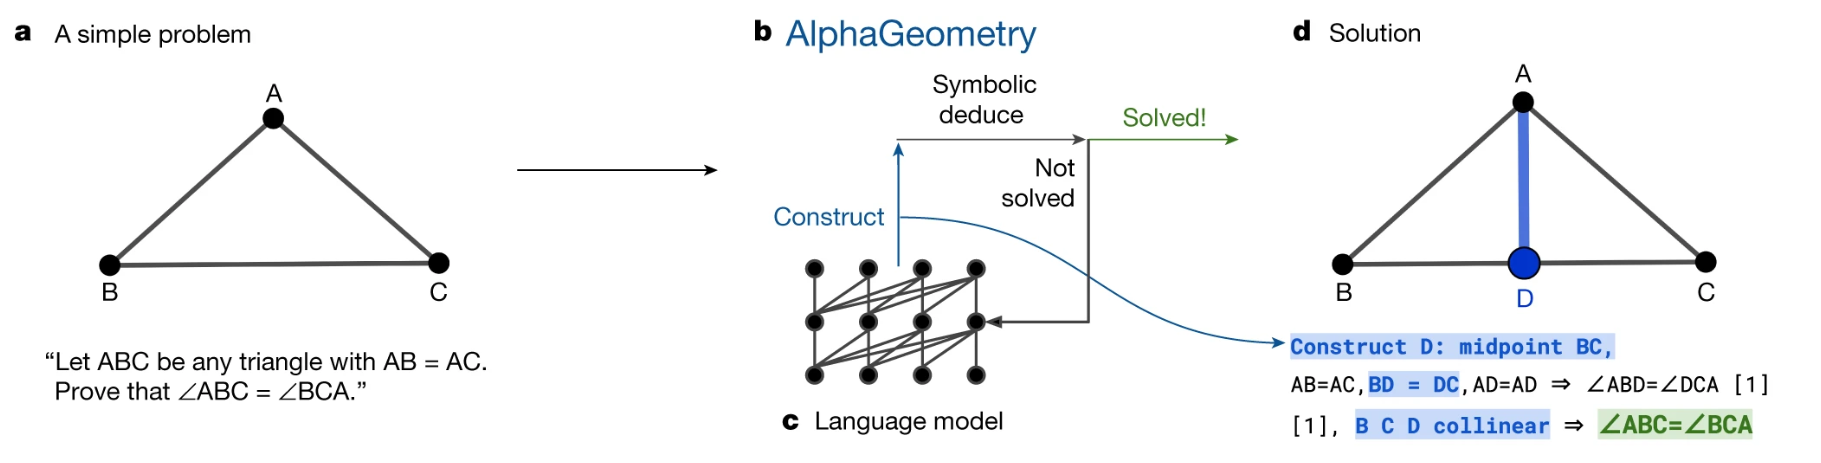
\includegraphics[width=17cm]{AlphaGeometry.png}
\end{center}
\caption{\label{fig:AlphaGeometry}
Funcionamento do \emph{AlphaGeometry}
(a) Um exemplo simples e seu diagrama. 
(b) AlphaGeometry inicia a busca de provas 
executando o mecanismo de dedução simbólica. 
O mecanismo deduz exaustivamente novas 
afirmações a partir das premissas do 
teorema até que o teorema seja provado 
ou novas afirmações sejam esgotadas. (c) 
Como o mecanismo simbólico não consegue 
encontrar uma prova, o modelo de 
linguagem constrói um ponto auxiliar, 
aumentando o estado da prova antes 
que o mecanismo simbólico tente novamente. 
O \emph{loop} continua até que uma solução seja 
encontrada. (d) Para este exemplo simples, 
o \emph{loop} termina após a primeira construção
 auxiliar ``$D$ como o ponto médio de $BC$''. 
(Fonte: \cite{trinh2024})}   
\end{figure*}

Mais recentemente, em 2024, o Google DeepMind anunciou o
desenvolvimento do \emph{AlphaGeometry}\cite{trinh2024},
 um sistema de inteligência
artificial capaz de resolver problemas complexos de
geometria em nível de Olimpíadas Internacionais de
Matemática (IMO). O \emph{AlphaGeometry} combina um modelo de
linguagem neural, que sugere construções geométricas
intuitivas, com um motor simbólico que verifica a
consistência lógica das etapas propostas. Em testes
realizados com 30 problemas geométricos da IMO (2000--2022),
o sistema resolveu 25, superando significativamente sistemas
anteriores, como o método de Wu \cite{chou1988},
que resolveu apenas 10, e aproximando-se do desempenho
médio de medalhistas de ouro humanos (25,9 problemas).

A abordagem do \emph{AlphaGeometry} ecoa, em espírito, os métodos
construtivos de Euclides, particularmente na utilização de
construções auxiliares, como adicionar pontos ou linhas para
facilitar a resolução de problemas geométricos. Assim como
Euclides empregava régua e compasso para construir figuras
que sustentassem suas provas, o \emph{AlphaGeometry} gera
construções geométricas auxiliares, validadas por um motor
simbólico que opera com regras lógicas formais. Esse
processo híbrido, combinando intuição neural e rigor
simbólico, representa uma ponte entre a tradição geométrica
euclidiana e as capacidades computacionais modernas
(Fig. \ref{fig:AlphaGeometry}).

Outra conquista recente possibilitada pelos
computadores são os programas de \emph{geometria
dinâmica}, como o GeoGebra, por exemplo, 
os quais permitem que as construções geométricas
sejam modificadas interativamente. Ficam aqui 
algumas indagações (um tanto anacrônicas, talvez):
Como Euclides, Arquimedes e Apolônio reagiriam
a tais ferramentas? Será que Sylvester 
teria uma melhor apreciação de Euclides se
tivesse experimentado o GeoGebra em sala de aula?
Quantas cores Byrne usaria em suas construções?

% A jornada dos \emph{Elementos}, da Alexandria helenística à
% inteligência artificial de ponta, ilustra a durabilidade e a
% adaptabilidade das ideias de Euclides. Enquanto os projetos
% de verificação formal buscam refinar o rigor lógico das
% provas euclidianas, o \emph{AlphaGeometry} demonstra como os
% princípios fundamentais da geometria euclidiana continuam a
% inspirar inovações, agora no domínio da inteligência
% artificial, redefinindo as fronteiras do raciocínio
% matemático automatizado.

\section{Historiografia}

Como discutido anteriormente, a análise da história
da matemática, enfrenta o desafio recorrente do anacronismo,
que consiste em interpretar obras do passado
à luz de padrões e conceitos
modernos. Pior do que isso, em muitos momentos,
a história da matemática foi escrita,
sobretudo por matemáticos,
numa perspectiva \emph{presentista} e \emph{paternalista},
ou seja, 
como se o historiador do presente, no cume do
progresso inevitável da matemática, observasse 
os antepassados tateando num labirinto de ideias turvas
que só ele agora pode compreender na totalidade.

Em um artigo incendiário, publicado em 1975,
o historiador Sabetai Unguru criticou 
abertamente essa perspectiva, 
argumentando que cada evento da história da 
matemática deve ser
compreendido em seus próprios termos, respeitando o contexto
filosófico, cultural e metodológico de sua época:
\begin{quote}
	É verdadeiramente deplorável e triste
quando um estudante da cultura e das
ideias antigas ou medievais deve
familiarizar-se primeiro com as noções
e operações da matemática moderna,
a fim de compreender o significado e a
intenção dos comentaristas modernos
que lidam com textos matemáticos
antigos e medievais.\cite{unguru1975}
\end{quote}
Esse artigo provocou uma grande polêmica,
da qual, pode-se dizer, Unguru saiu
vitorioso, pois desde então iniciou-se uma
tendência da história da matemática 
ser contada por historiadores profissionais,
e não mais por matemáticos tornados 
historiadores.


Mais recentemente, o debate historiográfico tem buscado um
equilíbrio. Em outro artigo igualmente inflamado,
publicado em 2014,
Viktor Blåsjö, questiona esse novo \emph{status quo}:
\begin{quote}
	Esta ``ortodoxia aceita'' molda o nosso
campo e, no entanto, raramente ou
nunca é submetida a uma análise crítica.
Na minha opinião, a autoimagem dos
historiógrafos modernos está muito
inflada. Neste artigo pretendo mostrar
que muitos dos argumentos a favor da
suposta superioridade da historiografia
moderna acabam por se resumir à
confusão, à convenção e à falta de
pensamento crítico, como se pode
esperar de um consenso que nunca foi
seriamente desafiado.\cite{blasjon2014}
\end{quote}
Essa perspectiva contemporânea propõe integrar
\emph{insights} matemáticos modernos para iluminar textos
históricos, sem desconsiderar seu contexto original. Esse
meio-termo reconhece que, embora 
seja crucial preservar a integridade histórica e filosófica do
período em que foram produzidas,
ferramentas modernas podem
esclarecer aspectos técnicos das obras antigas.
Assim, a historiografia da
matemática evolui em direção a uma abordagem que harmoniza o
rigor analítico com a sensibilidade contextual, permitindo
uma compreensão mais nuançada do legado de obras como 
\emph{Os Elementos}.
\section{Conclusão}

\emph{Os Elementos} de Euclides transcendem sua identidade como um
tratado de geometria da antiguidade, consolidando-se como um
pilar fundamental do pensamento ocidental. A genialidade da
obra reside em sua organização dedutiva sistemática, que
estabeleceu um paradigma para o raciocínio matemático que
perdurou por mais de dois milênios. Ao estruturar
proposições a partir de definições, postulados e noções
comuns, Euclides criou um modelo de argumentação lógica que
não apenas fundamentou a geometria, mas também influenciou
disciplinas tão diversas quanto o direito, a filosofia e a
programação de computadores. Essa abordagem, baseada na
derivação passo a passo de conclusões a partir de premissas
consensuais, tornou-se um alicerce do raciocínio
estruturado, evidenciando a universalidade e a
atemporalidade do método euclidiano.

Embora lógicos modernos identifiquem lacunas no sistema de
Euclides --- como suposições implícitas sobre continuidade
ou o uso de intuições visuais em diagramas ---, uma análise
contextual, especialmente sob a perspectiva dialética
proposta por Árpád Szabó, revela a riqueza da conquista de
Euclides. Longe de ser apenas um exercício de lógica formal,
\emph{Os Elementos} podem ser vistos como um empreendimento
dialético, enraizado na tradição grega de argumentação
estruturada, que visava estabelecer pontos de partida
acordados para o discurso geométrico. Essa interpretação
realça a sofisticação da obra em seu contexto histórico,
desafiando visões anacrônicas que julgam \emph{Os Elementos}
exclusivamente pelos padrões modernos.

A influência dos \emph{Elementos} estende-se por mais de dois mil
anos, moldando a matemática, a ciência e a filosofia. Desde
sua preservação por estudiosos do mundo islâmico até sua
redescoberta na Europa medieval, passando pelas inovações da
imprensa e pelas reformulações axiomáticas do século XIX, a
obra continuou a inspirar avanços intelectuais. No século
XXI, sua relevância persiste em campos como a inteligência
artificial, exemplificada pelo \emph{AlphaGeometry},
cuja abordagem construtiva ecoa os métodos
euclidianos. Assim,
o estudo dos \emph{Elementos}, o \emph{Farol de Euclides}, não apenas ilumina a história da
matemática, mas também projeta uma luz para a
exploração de novos caminhos.

\begin{figure}[b!]
\begin{center}
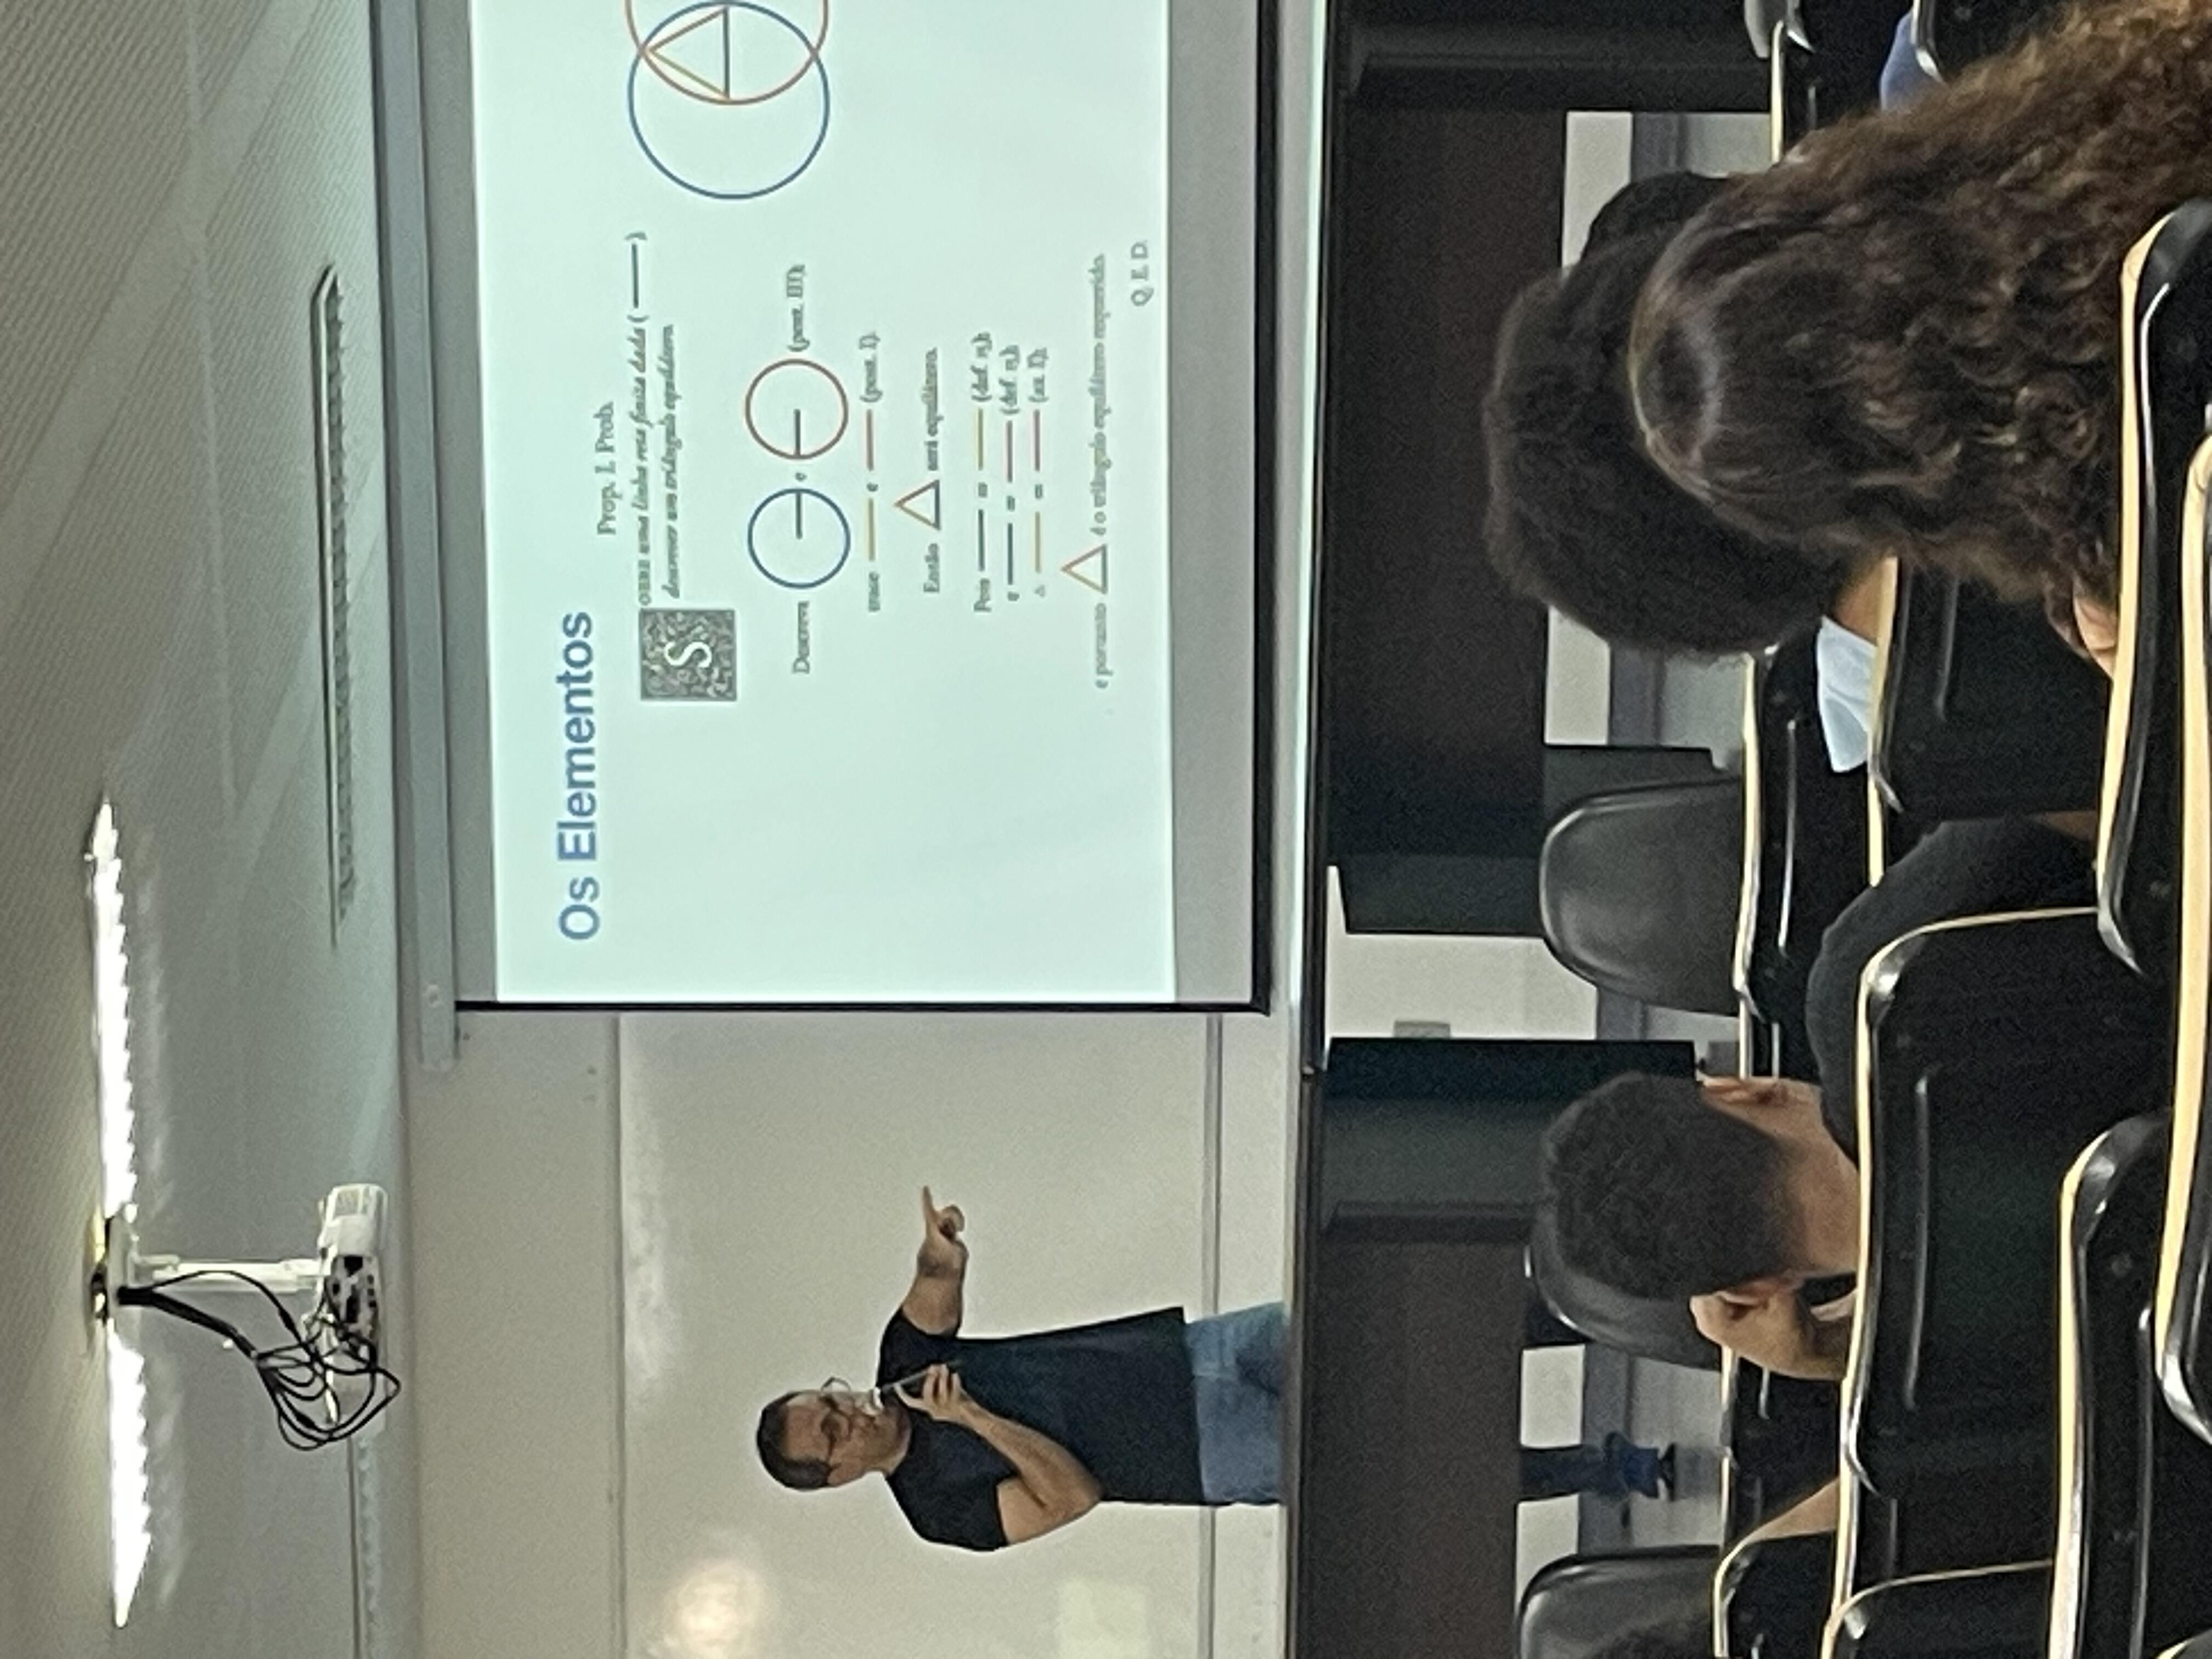
\includegraphics[width=9cm,angle=-90,origin=c]{palestra.jpg}
\end{center}
\caption{\label{fig:Palestra}
O autor durante a apresentação da palestra 
``O Farol de Euclides'' no Seminário 
Café Cultural.}
\end{figure}

%\nocite{*}
%\vfill

\bibliography{historia}


\vfill

% Mini bios 
% Seja informal e divertido
% Prefira fotos com fundo branco
\begin{wrapfigure}{L}{1.7cm}
\vspace{-10pt}
  
\includegraphics[width=2cm]{Vinicius.jpg}
\end{wrapfigure}\noindent
Vinícius Mello nasceu em Salvador e obteve seu doutorado
em Computação Gráfica no IMPA. Ensina matemática 
na UFBA e fica alegre sempre que pode usar o GeoGebra
em suas aulas. Gosta de matemática, música e programação 
em exata proporção, podendo ser encontrado a
(quase) qualquer momento fazendo ao menos uma dessas coisas.

\end{document}
